%%%%%%%%%%%%%%%%%%%%%%%%%%%%%%%%%%%%%%%%%
% University/School Laboratory Report
% LaTeX Template
% Version 3.1 (25/3/14)
%
% This template has been downloaded from:
% http://www.LaTeXTemplates.com
%
% Original author:
% Linux and Unix Users Group at Virginia Tech Wiki 
% (https://vtluug.org/wiki/Example_LaTeX_chem_lab_report)
%
% License:
% CC BY-NC-SA 3.0 (http://creativecommons.org/licenses/by-nc-sa/3.0/)
%
%%%%%%%%%%%%%%%%%%%%%%%%%%%%%%%%%%%%%%%%%

%----------------------------------------------------------------------------------------
%	PACKAGES AND DOCUMENT CONFIGURATIONS
%----------------------------------------------------------------------------------------

\documentclass{article}

\usepackage[version=3]{mhchem} % Package for chemical equation typesetting
\usepackage{siunitx} % Provides the \SI{}{} and \si{} command for typesetting SI units
\usepackage{graphicx} % Required for the inclusion of images
\usepackage{natbib} % Required to change bibliography style to APA
\usepackage{amsmath} % Required for some math elements 
\usepackage{listings}

\setlength\parindent{0pt} % Removes all indentation from paragraphs

\renewcommand{\labelenumi}{\alph{enumi}.} % Make numbering in the enumerate environment by letter rather than number (e.g. section 6)

%\usepackage{times} % Uncomment to use the Times New Roman font

%----------------------------------------------------------------------------------------
%	DOCUMENT INFORMATION
%----------------------------------------------------------------------------------------

\title{Golang Compiler\\ Final Report\\ Group 2} % Title


\date{\today} % Date for the report

\begin{document}

\maketitle % Insert the title, author and date

\begin{center}
\begin{tabular}{l r}
Members: & Shabbir Hussain \\ % Date the experiment was performed
& Ossama Ahmed \\ % Partner names
& Michael Ho \\ \end{tabular}
\end{center}

%----------------------------------------------------------------------------------------
%	SECTION 1
%----------------------------------------------------------------------------------------
\section{Introduction}
Our semester project was to build a go programming language compiler. Our compiler takes in source code from a subset of go called golite and compiles source code to jasmin code. The project requirements were to create a multi-stage compiler which:

\begin{itemize}
\item Scans source code for tokens and keywords
\item Parses the tokens according the grammar of golite into an Abstract Syntax Tree (AST)
\item Weeds the AST to comply with the grammar of golite
\item Type checks the source according to the typechecking rules of golite
\item Emits a pretty printed version of the source code
\item Emits a symbol table of the type-checked source
\item Code generates code in the target language (jasmin).
\end{itemize}

All the specifications of the golite language can be found at http://www.sable.mcgill.ca/~hendren/520/2016/.
This report will explain how we achieved the above mentioned requirements. 

\section{Compiler Structure}
Our compiler is built using the OCaml Lex and Menhir toolkit. We chose Ocaml for its strongly typed language in hopes to catch errors early in the development process. Furthermore, Ocaml contains many online help resources. Lastly, it is a great opportunity for hone our knowledge and programming skills in Ocaml. Ocamllex is tool for scanning the source into tokens which are encoded as Ocaml types. Menhir is the parser tool used to verify the syntax of the source code. The rest of the compiler is built using Ocaml native libraries. A high level overview of all the Ocaml modules, their inputs and their dependencies can be seen in figure \ref{fig:copmiler}. One of the design difficulties was the tight coupling of the AST to all the modules. This meant that if any changes were needed in the AST then all modules interacting with the AST had to change. As the project progressed, we often went back and changed the AST to add more information.

The rest of this section dives deeper into the design decisions of each module.

\begin{figure}[!h]
\centering
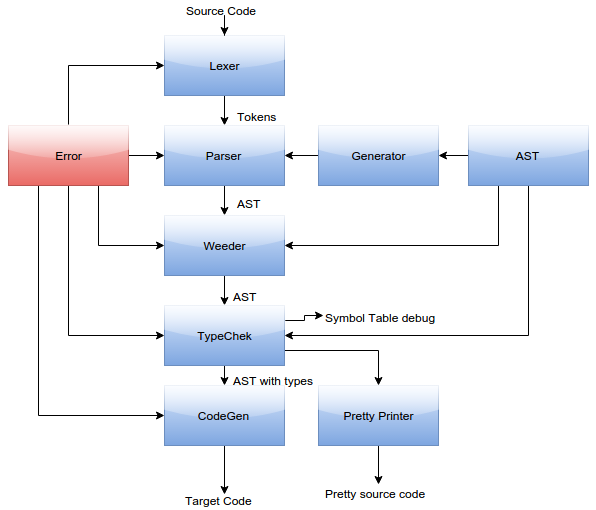
\includegraphics[width=1.0\textwidth]{compiler}
\caption{Overview of the modules in the compiler design}
\label{fig:copmiler}
\end{figure}

\subsection{Error Module}
We decided to have error messages standardized using an error module. By doing this all our error messages are of type GoliteError and contain the line number at which the error occurred.

\subsection{Abstract Syntax Tree}
The abstract syntax tree is composed of Ocaml Data Type. It is very close to the original golite grammar. We quickly realised that it would be advantageous to have each node hold the line number at which it occurred. This allowed us to give more detailed error messages when a parsing error occurs. Subsequently, it was useful in all the other phases as well or error checking. During type checking, we also added a field to every expression to contain type information. 

\subsection{Parsing Phase}
In order to have less dependency on the AST we decoupled the AST node constructors using a generate module. The generate module provided a standard interface for constructing the AST. The generator module proved its usefulness when we added a type field to the constructors of the AST. We only needed to change the generator code and not the parser. We initially construct the AST having all the type information set to empty in the generator module. 
One disadvantage of the generator is that it adds complexity to our code. To save time we considered the source code of our compiler as our documentation. However, to understand the AST received in the type-checker, we need to cross reference the AST with the parser and the generator. 

\subsection{Weeder}
We decided to place some syntactic checks in the weeding phase as opposed to the parser because it is easier to check. For example it is easier to check if  a switch statement has only one default case after all the cases have been defined. The parser builds the AST bottom up and our weeder checks the syntax from the top down. It searches trough every node until it hits a node that needs to propagate information to its leaf node. For example, a loop node needs to pass on information to its children that it is in a loop such that we can catch dangling break and continue statements. 

\subsection{Type checking Phase}
The type checker uses the same tree searching algorithm as the Weeder. We've implemented the type checking based on the specification on the sable course page as well as the reference compiler. We initially implemented the type checking as a two pass compiler in order to have function declarations with global scope since the go language allows it. We later removed this feature when verifying with the reference compiler. We added types to expressions in the AST such that we can print them for debugging purposes as well as code generating appropriate code. We decided to create constructors for each type to be included in the symbol table; this allows us to have a common interface for the symbol table. We also created a recursive type called symType. This allows us to create a "type" for structs which have structs in them.

\subsection{Pretty Printer}
For Pretty Printing, we decided to rewrite the PrettyPrinter using OCaml's imperative style (begin / end statements) and printing to stdout. Instead of printing as one large string as we did in milestone 1, now with imperative printing, it became easy to implement -pptype and soon code generation should be easier as well.

for the -dumpsymtab flag, the symtab file will be in the same folder as the executable
for the -pptype flag, the pptype file will be in the same folder as the source file

\subsection{Code Generation}
Our target language is jasmin. We initially chose jasmin because we believed we may be able to use the peephole optimizer in our compiler. Although it would have been interesting, this was not possible because we wanted to emit code that uses the full jasmin language; the peephole optimizer does not support floating point numbers. None the less, the exercise of the peephole optimizer allowed us to familiarize ourselves with jasmin code. 


We added some helpers to enable us to generate code to jasmin. We had a functions to 
\begin{itemize}
\item to start and end scope
\item to reference a variable name to a local
\item to get type checking information from the AST
\end{itemize}

Futhermore, some of the functionality of golite does not translate directly into jasmin. We had to implement some macros and algorithms in jasmin to accommodate these functionalities. The rest of this section will show detailed examples of these algorithms.

\subsubsection*{Structs}
We treat structs as java classes. Any time we encounter a struct we create a new file for the class defined by the struct. The class contains only public member fields.


The following struct
\begin{lstlisting}
type point3d struct{
    x,y,z int;
}
\end{lstlisting}
gets translated to the following class file
\begin{lstlisting}
.class public test1_struct_point3d
.super java/lang/Object

.field x I
.field y I
.field z I

.method public <init>()V
	.limit locals 99
	.limit stack 99
	aload_0
	invokenonvirtual java/lang/Object/<init>()V
	return
.end method
\end{lstlisting}

\subsubsection*{Append slices}
Golite allows slices to be dynamically changing arrays using the append() function. Since jasmin does not have dynamically changing arrays we decided to have an algorithm which creates a new array array with more space and then copies the values from the old array and finally, appends the new value. The golite code snippet corresponding to this is
\begin{lstlisting}
var x [] int;
var newValue int= 100;
x = append(x, newValue);
\end{lstlisting}
The algorithm described in java is 
\begin{lstlisting}[language=Java]
int x[]; //old array
int y[]; //new array
int newValue = 100;

y = new int[x.length];
System.arraycopy(x,0,y,0,x.length);
y[x.length] = newValue;
x=y;
\end{lstlisting}
The target jasmin code is as described below. The actual algorithm is generic for any local and type.
\begin{lstlisting}
aload_1 //old array ref in local 1
arraylength
iconst_1 
iadd
newarray int
dup //duplicate new array refernce
dup
dup
aload_1 // old array ref
swap
iconst_0 
swap
iconst_0
aload_1
arraylength	
invokestatic java/lang/System.arraycopy:(Ljava/lang/Object;ILjava/lang/Object;II)V
aload_1
arraylength
iload_2 //load new value
iastore //store in new array
astore_1 //store new array ref in local 1
\end{lstlisting}

\subsubsection*{If Else}
If else statements are tricky in jasmin. Our approach is to evaluate the entire conditional expression and put it on the stack. Then we check if that expression is 1 (true) or false. 


This code gen rule translates the below golite code
\begin{lstlisting}
	x := true
	y := false

	if y {
		//Do nothing
	} else if x {
		//Do nothing
	} else {
		println(x)
	}

\end{lstlisting}
Into the following jasmin code
\begin{lstlisting}
	iconst_1
	istore 0
	iconst_0
	istore 1
	iload 1
	ifne start1
	goto stop0
	start1:
	iload_0
	ifne start2
	goto stop0
	start2:
	getstatic java/lang/System/out Ljava/io/PrintStream;
	iload 0
	invokevirtual java/io/PrintStream/println(Z)V
	stop0:

\end{lstlisting}



\subsubsection*{Switch Statements}
Jasmin has a native command for switch statements called lookup switch. However, golite allows switch cases to have multiple case expressions. For this we implemented an evaluation algorithm that turns switch statements into big if/else cases. The algorithm puts the switch case expression on the stack and has each case expression check for equality. If the check passes the code branches into the statement list otherwise it goes to the next case. 

This code gen rule translates the below golite code
\begin{lstlisting}
	x := true
	y := 1

	switch y {
        case 1,2:
        x = false;
        default:
        x= true;
	}

\end{lstlisting}
into the following jasmin code
\begin{lstlisting}
	iconst_1
	istore 0
	ldc 1
	istore 1
	iload 1
 	dup
	ldc 1
	ifeq startcase1
	dup
	ldc 2
	ifeq startcase1
goto stopcase1
startcase1:
	iconst_0
	istore 0
	goto endSwitch
stopcase1:
	iconst_1
	istore 0
endSwitch:
	pop

\end{lstlisting}

\subsubsection*{Loops}
Loops are also similar to if/else statements except that we generate labels to the beggining and end of the loop. We pass the labels to the inner statement list such that a continue or break may goto the correct label. For any simple statements we evaluate them before the loop. Any increment statements get evaluated every loop at the end of the loop.

This code gen rule translates the below golite code
\begin{lstlisting}
 var y int;
    for i:=0;i<10;i++{
        y=i+1
    }

\end{lstlisting}
into the following jasmin code
\begin{lstlisting}
	iconst_0
	istore 0
	ldc 0
	istore 1
start0:
	iload 1
	ldc 10
	if_icmplt true1
	iconst_0
	goto stop1
	true1:
	iconst_1
	stop1:
	ifne stop0

	iload 1
	ldc 1
	iadd
	istore 0
	
	iload 1
	iconst_1
	iadd
	istore 1
	goto start0
stop0:


\end{lstlisting}

For full code examples of source compiled to target see the TESTPROGRAMS directory.

\section{Team Contribution}

\subsection{Shabbir Hussain}
Shabbir contributed to the:
\begin{itemize}
\item Parser for the Statements, If/else, switch case rules.
\item Milestone 1 report, Milestone 2 report, this document
\item Milestone 1,2 test cases and testing
\item Weeder to find if all paths have a return statement
\item Code Generation loops, statements, some expressions, append, 
\end{itemize}

\subsection{Ossama Ahmed}
For this project Sam served as the OCaml expert. 

\begin{itemize}
\item Milestone1: type declarations, expressions, variable declaration
\item Milestone2: 
\end{itemize}
	
\subsection{Michael Ho}


\section{Resources Used}
Some of the resources we used are: 

\begin{itemize}
\item https://gobyexample.com  
\item http://caml.inria.fr/pub/docs/manual-ocaml-4.00/manual026.html
\item https://realworldocaml.org/v1/en/html/parsing-with-ocamllex-and-menhir.html
\end{itemize}


\section{Conclusion and Future Work}
Building a compiler is a very large undertaking and in this section we want to discuss some of the lessons learned.


One of the most important lessons learned is the value of automated testing. Our first deliverable was lacking due to the fact that we missed many test cases. On the second deliverable we spent time designing a small test framework for our Ocaml project. The framework would compile the project and then run the compiler on hundreds of code examples testing for syntax, typecheking and code generation. This came in very handy no only to verify our work but also to have regression testing as we added features to the compiler. One draw back to this system is that the output to our test is a text file which needs to be manually verified. The manual verification takes a lot of time and understanding of how the test scripts are run. In the future it would be advantageous to also have automated verification in the testing framework such that the output of running passing tests is a green light and failing tests point to which tests failed. 


Another lesson learned is having all modules depend on the same AST is a terrible design choice. One change in the AST requires a change in all the dependant modules. In the future, it would be useful to design a tree search module which serves as an interface to the AST. This way, a change to the AST would only result in a change to the tree search module similar to our generator module. The reason we didn't implement this is because it was very easy to copy the tree searching code from the weeder to the pretty printer to the code-generator. 




%----------------------------------------------------------------------------------------


\end{document}